\documentclass[a4paper,11pt]{report}

% Document Setup
\usepackage[utf8]{inputenc}
\usepackage[T1]{fontenc}
\usepackage[french]{babel}

% Page Layout
\usepackage[top=3cm, bottom=3cm, left=3cm, right=3cm]{geometry}
\usepackage{fancyhdr}
\usepackage{indentfirst}

% Fonts and Text
\usepackage{csquotes}
\usepackage{enumitem}

% Mathematical Tools
\usepackage{amsfonts, amssymb, amsthm, amsmath, mathrsfs, array, stmaryrd}

% Tables
\usepackage{boldline, multirow, tabularx, colortbl, diagbox, makecell, booktabs}
\usepackage{siunitx} % For alignment and percentage formatting
\usepackage{graphicx} % Required for \resizebox

\sisetup{
    round-mode=places, % Rounds numbers
    round-precision=2, % to 2 decimal places
    table-format=2.2\%, % Aligning by decimal points
    table-space-text-post=\%, % Ensuring space for the percent sign
}

% Graphics and Colors
\usepackage{pgf, tikz, xcolor}
\usetikzlibrary{calc, positioning, shapes.geometric, shapes.symbols, shapes.misc, fit, calc, shapes, arrows, arrows.meta, fadings, through}

% Hyperlinks and PDF Handling
\usepackage{hyperref}
\usepackage{pdfpages}

% Listings and Algorithms
\usepackage{listings, algorithm2e}
\usepackage{algpseudocode}
\usepackage{enumitem} 

% Date and Time
\usepackage[nodayofweek, level]{datetime}

% Additional Tools
\usepackage{ifluatex}
\usepackage{notoccite}
\usepackage{appendix}
\usepackage{fancybox}
\usepackage[backend=biber, sorting=none, style=alphabetic]{biblatex}
\addbibresource{refs/bibliography.bib}
\usepackage[printonlyused]{acronym}
\usepackage{caption}
\usepackage{float}

% Forestry and Directory Trees
\usepackage{dirtree}
\usepackage{forest}
\usepackage{amssymb}

% Custom Definitions
\newtheorem{definition}{Definition}

% Input Files
% \newcommand{\addstudent}[4]{\textbf{#1} \\ #2 \\ #3 \\ \href{mailto:#3?subject=Regarding\projecttitle}{#4}\\}
\newcommand{\addstudent}[1]{\textbf{#1} \\}
\newcommand{\addtutor}[2]{#1 \\ #2\\}
\newcommand{\addentity}[2]{\textbf{#1} & #2\\}
\newcommand{\supervisor}{Raca TODOSIJEVIC - A/Prof}
\newcommand\blankpage{%
    \null
    \thispagestyle{empty}%
    \addtocounter{page}{-1}%
    \newpage}


%=========================================================================

% Complétez ici le titre de votre projet :
\def\projecttitle{
    Graphes et Optimisation : Recherche du plus court chemin et Problème du voyageur de commerce
}
% Complétez ici le titre de votre prénom et votre nom :
\def\students{
    % \addstudent{Elias BOULANGER}{INSA Hauts-de-France - ICY}{Université Polytechnique Hauts-de-France}{elias.boulanger@uphf.fr}
    % \addstudent{Thomas AUBERT}{INSA Hauts-de-France - ICY}{Université Polytechnique}{thomas.aubert1@uphf.fr}
    \addstudent{Elias BOULANGER}
    \addstudent{Thomas AUBERT}
}

% Complétez ici votre département (décommentez la ligne correspondante) :
\def\departement{
    Département d'Informatique et de Cybersécurité
}
\newcommand\tab[1][0.6cm]{\hspace*{#1}} %Create and define tab

\definecolor{lightgray}{gray}{0.85}
\definecolor{verylightgray}{gray}{0.85}

\newcolumntype{L}[1]{>{\raggedright\arraybackslash\hspace{0pt}}p{#1}}
\newcolumntype{R}[1]{>{\raggedleft\arraybackslash\hspace{0pt}}p{#1}}
\newcolumntype{C}[1]{>{\centering\arraybackslash\hspace{0pt}}p{#1}}

\renewcommand\thesection{\arabic{section}}
\renewcommand\thesubsection{\thesection.\arabic{subsection}}

% Redefine plain style, which is used for titlepage and chapter beginnings
% From https://tex.stackexchange.com/a/30230/828
\fancypagestyle{plain}{%
    \renewcommand{\headrulewidth}{0pt}%
    \fancyhf{}%
    \fancyfoot[R]{\thepage}%
}



%------- Do not append new commands after :

\hypersetup{	
    colorlinks=false, % colorise les liens
    linkbordercolor={1 1 1},
    breaklinks=true, % permet le retour à la ligne dans les liens trop longs
    urlcolor=blue, % couleur des hyperliens 
    linkcolor=black,	% couleur des liens internes 
    citecolor=black,	% couleur des références 
    pdftitle={Graphes et Optimisation : Recherche du plus court chemin et Problème du voyageur de commerce}, % informations apparaissant dans 
    pdfauthor={Elias Boulanger, Thomas Aubert}, % les informations du document 
    pdfsubject={}	% sous Acrobat. 
}
\title{Graphes et Optimisation : Recherche du plus court chemin et Problème du voyageur de commerce\\ \vspace{0.5cm} \LARGE{\textbf{\projecttitle}} \vspace{0.75cm}}
\author{\students \\ \vspace{1cm} \\ Superviseur : \tutor}
\date{\today}
\RequirePackage{fancyhdr}
\pagestyle{fancy}
\renewcommand{\headrule}{}
\lhead{}
\chead{}
\rhead{}
\lfoot{}
\cfoot{}
\rfoot{\thepage}

% Set the font size for the cover page to 12pt
\fontsize{12pt}{14pt}\selectfont

\AtBeginDocument{\pagenumbering{gobble}
%\makeatletter
\noindent\begin{tikzpicture}[remember picture, overlay, shift={(current page.south west)}]
    %Images
    \node[anchor=north west] at (2.45,23.7) {
\includegraphics[height=1.6cm, keepaspectratio]{cover/meta/insa-logo.png}};
    \node[anchor=north east] at (18.55,23.8) {
\includegraphics[height=1.8cm, keepaspectratio]{cover/meta/uphf-logo.png}};

    \node[above = 280pt of current page.center] (rapport) {
        \begin{tabular}{c}
            \huge{\textsc{\textbf{I}nstitut \textbf{N}ational des \textbf{S}ciences \textbf{A}ppliquées}} \\ \huge{\textsc{des \textbf{H}auts-de-\textbf{F}rance}}
        \end{tabular}
    };
        
    % Textes
    \node[below = 10pt of current page.center] (ptitle) {\parbox{\textwidth}{\centering\huge{\textsc{\projecttitle}}}};
    \node[above = 12.5pt of ptitle.north] {\rule{15cm}{0.25mm}};
    \node[below = 12.5pt of ptitle.south] {\rule{15cm}{0.25mm}};
    
    \node[above = 90pt of ptitle] {\LARGE{\textbf{\departement}}};
    
    \node[above = 40pt of ptitle] {\huge{\textsc{\textbf{Rapport des Travaux Pratiques}}}};

    % Adding the Supervisor Title and Name just below the Date of defence
    \node[below = 5pt of ptitle, xshift = 1.3cm] at (14.7, 10) (pdate){\large{\textbf{Date:} \today}};
    \node[below = 5pt of pdate, xshift = -2.3cm] (supervisorstitle) {\large{\textbf{Professeur:} \supervisor}};
    
    \node[anchor = south west, xshift = 0.65cm] at (2,2) (pstudents) {\large{\centering\begin{tabular}{lllll}\students\end{tabular}}};
\end{tikzpicture}

\newpage
% \blankpage}

\AtEndDocument{\input{cover/cover_out.tex}}

% Reset the font size to 11pt
\fontsize{11pt}{13pt}\selectfont

\begin{document}

\newpage
\thispagestyle{empty}
\tableofcontents

\newpage
\chapter*{Liste des Acronymes}
\label{chap:acronymes}

\begin{acronym}
    % \acro{<acronyme>}{<signification>}
    \acro{IA}{Intelligence Artificielle}
    \acro{LSB}{Bit de Poids Faible}
    \acro{MSB}{Bit de Poids Fort}
    \acro{PdV}{Point de Vue}
    \acro{TP}{Travail Pratique}
\end{acronym}

\newpage
\thispagestyle{empty}
\listoffigures
\listoftables

\newpage
\pagenumbering{arabic}

\chapter{Introduction}
\label{chap:introduction}
Dans le domaine de l'informatique et de la cybersécurité, l'étude de la théorie des graphes et de l'optimisation joue un rôle crucial, en particulier pour résoudre des problèmes complexes de routage et de recherche de chemin. Ce rapport se penche sur deux problèmes classiques dans ce domaine : le problème du plus court chemin et le problème du voyageur de commerce. Ces problèmes sont non seulement fondamentaux pour la recherche théorique mais ont également des applications pratiques significatives dans des domaines tels que le routage des réseaux, la logistique et la robotique. Ce travail pratique vise à explorer des solutions algorithmiques efficaces pour ces problèmes, en utilisant des approches classiques et heuristiques. Ce rapport détaille la structure du projet, les méthodologies employées, l'implémentation en Python et une analyse comparative des résultats obtenus à partir de différentes stratégies algorithmiques.
\newpage

\chapter{Structure du projet}
\label{chap:structure}

Dans ce chapitre, nous décrivons la structure de données et les choix techniques effectués pour la représentation et la manipulation des graphes utilisés dans ce TP. Nous implémentation se construit autour de deux types de problèmes : le problème du plus court chemin et le problème du voyageur de commerce.

\section{Représentation des noeuds}
Nous avons choisi de représenter chaque noeud du graphe à l'aide d'une classe \texttt{Node}. Cette classe contient les informations nécessaires pour les algorithmes de recherche de chemin et les fonctions associées. Voici la description des attributs principaux :

\begin{itemize}
    \item \textbf{position} : Un tuple \texttt{(x, y)} représentant les coordonnées du noeud dans le réseau.
    \item \textbf{neighbors} : Un dictionnaire où les clés sont des directions \texttt{(dx, dy)} et les valeurs sont les noeuds voisins correspondants. Cela permet de naviguer efficacement dans le graphe.
    \item \textbf{parent} : Le noeud parent, utilisé pour reconstruire le chemin après l'exécution de l'algorithme A*.
    \item \textbf{is\_obstacle} : Un booléen indiquant si le noeud est un obstacle (non praticable). Les noeuds obstacles ne peuvent pas être voisins d'autres noeuds. Permet une structure de graphe dynamique.
    \item \textbf{g, h, f} : Ces attributs sont utilisés dans l'algorithme A*. \texttt{g} est le coût du chemin depuis le noeud de départ, \texttt{h} est une estimation heuristique du coût pour atteindre la destination, et \texttt{f} est la somme des deux (\texttt{f = g + h}).
\end{itemize}

\section{Représentation du graphe}
La classe \texttt{Graph} est utilisée pour représenter et manipuler le graphe. Elle gère deux types de problèmes : le problème du plus court chemin et le problème du voyageur de commerce.

\subsection{Attributs principaux}
\begin{itemize}
    \item \textbf{start, objective} : Les noeuds de départ et d'arrivée pour le problème du plus court chemin.
    \item \textbf{graph} : Une matrice de noeuds utilisée pour le problème du plus court chemin. Notre (0, 0) est la node en haut à gauche du graphe, pour faciliter la manipulation et visualisation lignes/colonnes.
    \item \textbf{node\_list} : Une liste de noeuds utilisée pour le problème du voyageur de commerce.
    \item \textbf{cost} : Un dictionnaire où les clés sont des tuples de noeuds et les valeurs sont les coûts des arêtes entre ces noeuds.
    \item \textbf{shape} : Les dimensions du graphe. La valeur est dynamique, initialisée lors de la lecture du fichier d'entrée. Si les dimensions du graphe sont modifiés, cette valeur est alors mise à jour.
    \item \textbf{file\_path, problem} : Le chemin vers le fichier d'entrée et le type de problème à résoudre.
\end{itemize}

Remarque : la présence de deux structures de graphes, \texttt{node\_list}, et \texttt{graph} s'explique par la différence de représentation des noeuds pour les deux problèmes. Pour le problème du plus court chemin, nous utilisons une matrice de noeuds pour faciliter l'implémentation des algorithmes de recherche, notamment CPLEX. Dans ce cas, les couts sont directement dépendant de coordonnées. Pour le problème du voyageur de commerce, nous utilisons une liste de noeuds pour faciliter la manipulation des ensembles de noeuds. Dans ce cas, les couts sont définis par l'utilisateur, il n'y a pas de dépendance directe avec les coordonnées.

\subsection{Méthodes principales}
\begin{itemize}
    \item \textbf{add\_node} : Ajoute un noeud au graphe. Pour le problème du plus court chemin, le graphe est étendu si nécessaire. Pour le problème du voyageur de commerce, le noeud est simplement ajouté à la liste.
    \item \textbf{add\_edge} : Ajoute une arête entre deux noeuds avec un coût spécifié. Cette méthode vérifie également que les noeuds sont voisins dans le problème du plus court chemin.
    \item \textbf{remove\_node} : Marque un noeud comme obstacle et déconnecte ses voisins.
    \item \textbf{solve} : Résout le problème spécifié en utilisant l'algorithme A* pour le plus court chemin ou une méthode d'énumération pour le voyageur de commerce.
    \item \textbf{get\_neighbors} : Retourne les voisins d'un noeud donné. Prend en compte les obstacles et les limites du graphe.
    \item \textbf{get\_edges} : Retourne une liste de toutes les arêtes du graphe.
\end{itemize}

Remarque : les méthodes \texttt{add\_node}, \texttt{add\_edge}, et \texttt{remove\_node} sont implémentées pour les deux types de problèmes mais ne sont pas utilisées au sein du projet. Elles sont utiles si l'on veut manipuler dynamiquement le graphe ; ce qui est possible, mais n'a pas été necessaire pour les problèmes traités dans ce TP. Lorsque nous avions besoin de créer un graphe, nous initialisions les variables nécessaires via le traitement du fichier d'entrée.

\section{Choix de performance et praticité}
\begin{itemize}
    \item \textbf{Utilisation de dictionnaires pour les voisins} : Cette structure permet un accès rapide et une gestion efficace des voisins d'un noeud.
    \item \textbf{Matrice de noeuds} : Pour le problème du plus court chemin, cette représentation facilite l'implémentation des algorithmes de recherche et de parcours.
    \item \textbf{Liste de noeuds} : Pour le problème du voyageur de commerce, cette représentation est plus adaptée car elle permet de manipuler facilement les ensembles de noeuds.
    \item \textbf{Coûts des arêtes} : Les coûts sont calculés à partir de la distance euclidienne pour le problème du plus court chemin, ce qui permet une estimation réaliste des distances. Pour le problème du voyageur de commerce, les coûts sont définis par l'utilisateur dans le fichier d'entrée.
\end{itemize}


\section{Exécution du programme}
Pour exécuter le programme, nous utilisons le fichier \texttt{main.py} qui contient les fonctions principales pour lancer les différents algorithmes sur les problèmes spécifiés. Voici une explication détaillée de la fonction principale et de son utilisation :

\begin{itemize}
    \item \textbf{run} : Cette fonction exécute l'algorithme spécifié sur le problème donné. Les paramètres incluent le nombre d'itérations (\texttt{n\_iter}), le type de problème (\texttt{problem}), l'algorithme à utiliser (\texttt{algo}), le chemin du fichier d'entrée (\texttt{file\_path}), et des options pour afficher (\texttt{display}), sauvegarder (\texttt{save}), ou afficher les détails (\texttt{verbose}) du résultat. La fonction génère d'abord le graphe à partir du fichier spécifié, puis exécute l'algorithme et mesure le temps d'exécution pour chaque itération.
    \item \textbf{compare\_algo} : Cette fonction compare les temps d'exécution des algorithmes A* et CPLEX pour le problème du plus court chemin, ou des algorithmes de force brute et CPLEX pour le problème du voyageur de commerce. Si un chemin de fichier est spécifié, la résolution est effectuée sur ce fichier, sinon un graphe aléatoire est généré.
\end{itemize}

Pour exécuter le programme, ouvrez un terminal et utilisez la commande suivante :

\begin{verbatim}
python main.py
\end{verbatim}

Les modules python nécessaires sont spécifiés dans le fichier \texttt{requirements.txt}. Le module \texttt{docplex} est requis mais n'est pas dans le fichier car la licence pro ou académique est nécessaire pour résoudre les problèmes de plus de 30 noeuds.
\newpage

\chapter{Plus court chemin}
\label{ch:shortest_path}

\section{Modélisation}
\label{sec:shortest_path_model}

On considère un graphe non orienté $G=<S,A>$ où $S$ est l'ensemble des sommets et $A$ l'ensemble des arêtes. Chaque arête $a_{ij}$ est associée à un coût $c_{ij}$, qui vaudra 1 dans le cas où deux sommets sont reliés horizontalement ou verticalement, et $\sqrt{2}$ dans le cas où ils sont reliés en diagonale. On cherche à déterminer le plus court chemin entre un sommet de départ $s$ et un sommet d'arrivée $t$.

\subsection{Variables}

\begin{itemize}
    \item $x_{ij}$ : vaut 1 si l'arête $a_{ij}$ est empruntée, 0 sinon
\end{itemize}

\subsection{Fonction objectif}

On cherche à minimiser la somme des coûts des arêtes empruntées :

\begin{equation}
    \min \sum_{(i,j) \in A} c_{ij} \cdot x_{ij}
\end{equation}

\subsection{Contraintes}

\begin{itemize}
    \item Le sommet de départ $s$ est toujours relié à un sommet :
    \begin{equation}
        \sum_{j \in S} x_{sj} = 1
    \end{equation}
    \item De même, le sommet d'arrivée $t$ est toujours relié à un sommet :
    \begin{equation}
        \sum_{i \in S} x_{it} = 1
    \end{equation}
    \item Le sommet de départ $s$ n'a pas d'arête entrante :
    \begin{equation}
        \sum_{i \in S} x_{is} = 0
    \end{equation}
    \item De même, le sommet d'arrivée $t$ n'a pas d'arête sortante :
    \begin{equation}
        \sum_{j \in S} x_{tj} = 0
    \end{equation}
    \item Chaque sommet a le même nombre d'arêtes entrantes et sortantes (sauf $s$ et $t$):
    \begin{equation}
        \sum_{j \in S} x_{ij} = \sum_{j \in S} x_{ji} \quad \forall i \in S \setminus \{s,t\}
    \end{equation}
    \item Notre graphe n'étant pas orienté, nous devons empêcher les sous-cycles, c'est-à-dire le cas où on trouve une arête $a_{ij}$ et une arête $a_{ji}$ dans le chemin :
    \begin{equation}
        \sum_{(i,j) \in A} x_{ij} + \sum_{(j,i) \in A} x_{ji} \leq 1 \quad \forall i,j \in S \setminus \{s,t\}
    \end{equation}
\end{itemize}

Nous avons implémenté et résolu ce problème en Python, en utilisant la librairie \texttt{docplex.mp.model} de CPLEX. Le code complet est disponible en annexe \ref{app:shortest_path_code}.

\section{A Star}
\label{sec:shortest_path_astar}

L'algorithme A* est une méthode heuristique utilisée pour trouver le plus court chemin entre deux sommets dans un graphe. Il combine les avantages de la recherche en profondeur et de la recherche en largeur tout en utilisant une fonction heuristique pour guider la recherche. Voici une description du pseudo-code de base de l'algorithme A* et des améliorations apportées.

\subsection{Pseudo-code de base}
Le pseudo-code de base de l'algorithme A* est le suivant :
\begin{enumerate}
    \item Initialiser l'ensemble ouvert (open set) avec le noeud de départ.
    \item Initialiser le coût g du noeud de départ à 0.
    \item Calculer la valeur heuristique h pour le noeud de départ et mettre à jour sa valeur f (f = g + h).
    \item Répéter jusqu'à ce que l'ensemble ouvert soit vide :
    \begin{enumerate}
        \item Extraire le noeud avec la plus petite valeur f de l'ensemble ouvert.
        \item Si ce noeud est le noeud d'arrivée, reconstruire le chemin en remontant à travers les parents.
        \item Pour chaque voisin du noeud courant :
        \begin{enumerate}
            \item Calculer le coût g temporaire pour ce voisin.
            \item Si ce coût g est inférieur au coût g actuel du voisin, mettre à jour les valeurs g, h et f du voisin, et définir le noeud courant comme parent du voisin.
            \item Ajouter le voisin à l'ensemble ouvert s'il n'y est pas déjà.
        \end{enumerate}
    \end{enumerate}
\end{enumerate}

Pour que cet algorithme fonctionne, il ne faut pas oublier d'initialiser la valeur g des noeuds à l'infini. Aussi, il faudrait réinitialiser les valeurs g, h et f des noeuds à l'infini à chaque itération de l'algorithme. Cela permet de recalculer les valeurs g, h et f correctement pour chaque itération.

\subsection{Améliorations}
\subsubsection*{Avec une heap queue}
Pour améliorer l'efficacité de l'algorithme A*, nous utilisons une file de priorité (heap queue) pour l'ensemble ouvert. Cela permet d'extraire le noeud avec la plus petite valeur f en temps logarithmique. Les voisins des noeuds sont initialisés une seule fois au début du programme, ce qui réduit le coût de recalcul des voisins à chaque itération.

\subsubsection*{Avec un ensemble de noeuds visités}
Pour réduire la vérification de présence d'un noeud dans l'ensemble ouvert, nous utilisons un ensemble (set en python) pour suivre les noeuds déjà visités. Cela permet de vérifier si un noeud est dans l'ensemble ouvert en temps constant.

\subsection{Implémentation en Python}
Les optimisations se traduisent dans le code Python suivant :

\begin{verbatim}
def a_star(start_node: Node, end_node: Node) -> Optional[List[Node]]:
    open_set = [start_node]
    heapq.heapify(open_set)
    opens_set_tracker = {start_node}

    start_node.g = 0
    start_node.h = heuristic(start_node, end_node)
    start_node.f = start_node.h

    while open_set:
        current_node: Node = heapq.heappop(open_set)
        opens_set_tracker.remove(current_node)

        if current_node == end_node:
            return reconstruct_path(current_node)

        for neighbor in current_node.neighbors.values():
            tentative_g = current_node.g + distance(current_node, neighbor)
            if tentative_g < neighbor.g:
                neighbor.parent = current_node
                neighbor.g = tentative_g
                neighbor.h = heuristic(neighbor, end_node)
                neighbor.f = neighbor.g + neighbor.h
                if neighbor not in open_set_tracker:
                    heapq.heappush(open_set, neighbor)
                    opens_set_tracker.add(neighbor)

    return None
\end{verbatim}

Remarque : les fonctions \texttt{heuristic}, \texttt{distance}, et \texttt{reconstruct\_path} sont des fonctions auxiliaires utilisées dans l'algorithme A*. Les deux premières permettent une flexibilité dans le calcul des coûts et des heuristiques, tandis que la dernière permet de reconstruire le chemin à partir du noeud d'arrivée via les parents. Par défaut une bonne mesure de distance est la distance de Manhattan, et une bonne heuristique est la distance euclidienne. Cette dernière permet le déplacement en diagonale. Nous n'utilisons pas la distance euclidienne pour le cout de déplacement, car elle favorise une augmentation du nombre de noeuds visités et donc une augmentation du temps de calcul.

\subsection{Optimisation spatiale et temporelle}
L'algorithme A* n'utilise pas l'ensemble complet de la matrice du graphe, mais uniquement les noeuds de départ et d'arrivée ainsi que les voisins nécessaires pour chaque itération. Cela permet d'optimiser l'utilisation de la mémoire et d'accélérer les opérations.

Les voisins des noeuds sont stockés dans un attribut de chaque noeud et initialisés une seule fois au début du programme. Ainsi, chaque résolution de A* n'appelle pas de fonctions \texttt{get\_neighbors}, mais opère directement sur l'attribut \texttt{neighbors} de chaque noeud.

\subsection{Complexité de l'algorithme A*}

\subsubsection*{Complexité temporelle sans heap queue}
Sans l'utilisation de heap queue, l'ensemble des nœuds ouverts (open set) est géré comme une liste non ordonnée. Les opérations de recherche du nœud avec le coût \( f \) minimal et l'insertion d'un nouveau nœud sont coûteuses :

\begin{itemize}
    \item Extraction du nœud avec le coût \( f \) minimal :$\mathcal{O}(n)$
    \item Insertion d'un nouveau nœud : $\mathcal{O}(1)$
    \item Vérification de la présence dans open set : $\mathcal{O}(n)$
\end{itemize}

La complexité temporelle totale est alors \( O(E \cdot V) \), où \( E \) est le nombre d'arêtes et \( V \) est le nombre de nœuds.

\subsubsection*{Complexité temporelle avec heap queue}
Avec l'utilisation de heap queue, l'ensemble des nœuds ouverts (open set) est géré comme une heap binaire. Cela optimise les opérations suivantes :

\begin{itemize}
    \item Extraction du nœud avec le coût \( f \) minimal : $\mathcal{O}(\log n)$
    \item Insertion d'un nouveau nœud : $\mathcal{O}(log n)$
    \item Vérification de la présence dans open set : $\mathcal{O}(n)$
\end{itemize}

Même si la vérification de la présence reste coûteuse, les opérations de base de l'algorithme, à savoir l'extraction et l'insertion dans la heap, dominent la complexité globale. La complexité temporelle totale est donc $\mathcal{O}(E \log V)$.

\subsubsection*{Complexité temporelle avec heap queue et ensemble (set)}
En ajoutant un ensemble (set) pour suivre les nœuds dans open set, on optimise la vérification de la présence :

\begin{itemize}
    \item Extraction du nœud avec le coût \( f \) minimal : $\mathcal{O}(\log n)$
    \item Insertion d'un nouveau nœud : $\mathcal{O}(\log n)$
    \item Vérification de la présence dans open set : $\mathcal{O}(1)$
\end{itemize}

Cependant, ces améliorations ne changent pas la complexité dominante de l'algorithme. L'opération d'extraction du nœud avec le coût \( f \) minimal et l'insertion dans la heap binaire restent les opérations les plus coûteuses et se produisent $\mathcal{O}(E)$ fois. Par conséquent, la complexité temporelle totale reste $\mathcal{O}(E \log V)$.

\subsubsection*{Note}
La complexité temporelle - $\mathcal{O}(E \log V)$ ou $\mathcal{O}(E \cdot V)$ - est une borne supérieure. En pratique, à moins qu'il n'existe aucun chemin entre les deux nœuds, et pour une bonne heuristique, la complexité temporelle est bien plus faible.


\section{Génération de graphes aléatoires}
\label{sec:shortest_path_random_graph}

Afin de pouvoir comparer les deux implémentations, nous avons créé une fonction générant des graphes aléatoires. Cette fonction prend en paramètre le nombre de sommets $n$ et la probabilité $p$ qu'un sommet soit un obstacle.

\begin{figure}[H]
    \centering
    \begin{includegraphics}[width=1\textwidth]{resources/gen_path_graph.png}
    \end{includegraphics}
    \caption{Fonction générant un graphe aléatoire}
    \label{fig:gen_path_graph}
\end{figure}

\section{Résultats et comparaison des deux implémentations}
\label{sec:shortest_path_comparison}

Les deux méthodes étant fondamentalement différentes, nous pouvons observer de légères différences sur les résultats obtenus.

Les graphiques suivants représentent le réseau de sommets liés par des arêtes, avec le sommet de départ en vert, le sommet d'arrivée en bleu clair, et le chemin trouvé en rouge.

Nous avons une légère différence dans le chemin trouvé par CPLEX et A Star sur le réseau \texttt{reseau\_20\_20\_1}:

\begin{figure}[H]
    \centering
    \begin{includegraphics}[width=.6\textwidth]{resources/20_20_cplex.png}
    \end{includegraphics}
    \caption{Graphique de la solution trouvée par CPLEX}
    \label{fig:cplex_2020}
\end{figure}

\begin{figure}[H]
    \centering
    \begin{includegraphics}[width=.6\textwidth]{resources/20_20_astar.png}
    \end{includegraphics}
    \caption{Graphique de la solution trouvée par A Star}
    \label{fig:astar_2020}
\end{figure}

\subsection{Comparaison des temps de calcul}
\begin{table}[H]
    \centering
    \begin{tabular}{|c|c|c|c|c|c|}
        \hline
        \textbf{Méthode / Taille du graphe} & 10 & 15 & 30 & 60 & 120 \\
        \hline
        \textbf{A*} & 0.02184 & 0.00013 & 0.00051 & 0.00248 & 0.00804s \\
        \hline
        \textbf{CPLEX} & 0.00009 & 0.04013 & 0.19364 & 0.56905 & 2.36712s \\
        \hline
    \end{tabular}
    \caption{Temps d'exécution (s) des deux méthodes en fonction de la taille du graphe. Moyenne obtenue sur 100 itérations. Densité des arêtes : 0.3}
\end{table}

n= 500, p=0.3
h=0 : 0.00965s
h=euclidienne : 0.01021s
h=manhattan : 0.01002s
\newpage

\chapter{Problème du voyageur de commerce}
\label{chap:tsp}

Le problème du voyageur de commerce (TSP) consiste à trouver le plus court chemin passant par chaque ville une et une seule fois, et revenant à la ville de départ. Nous allons employer deux méthodes pour résoudre ce problème : une résolution linéaire avec CPLEX \cite{wiki_tsp} et une résolution par énumération des permutations possibles.

\section{Modélisation}
\label{sec:tsp_model}
On considère un graphe non orienté $G=<S,A>$ où $S$ est l'ensemble des sommets et $A$ l'ensemble des arêtes. À chaque arête $a_{ij}$ est associée une distance $c_{ij}$. On cherche à déterminer le plus court chemin passant par chaque sommet une et une seule fois, et revenant au sommet de départ.

\subsection*{Variables}

\begin{itemize}
    \item $x_{ij}$ : vaut 1 si l'arête $a_{ij}$ est empruntée, 0 sinon
\end{itemize}

\subsection*{Fonction objectif}

On cherche à minimiser la somme des distances des arêtes empruntées :

\begin{equation}
    \min \sum_{(i,j) \in A} c_{ij} \cdot x_{ij}
\end{equation}

\subsection*{Contraintes}

\begin{itemize}
    \item Chaque sommet doit être relié à une arête entrante :
    
    \begin{equation}
        \sum_{i \in S} x_{ik} = 1 \quad \forall k \in S
    \end{equation}
        

    \item Chaque sommet doit être relié à une arête sortante :
    
    \begin{equation}
        \sum_{j \in S} x_{kj} = 1 \quad \forall k \in S
    \end{equation}

    \item Empêcher les sous-cycles :
    
    \begin{equation}
        \sum_{(i,j) \in A} x_{ij} + \sum_{(j,i) \in A} x_{ji} \leq 1 \quad \forall i,j \in S
    \end{equation}
\end{itemize}

Le code Python équivalent à ce modèle est donné en annexe \ref{app:tsp_model}.

\section*{Résolution par énumération}

On peut résoudre le problème du TSP en énumérant toutes les permutations possibles des villes, et en calculant la distance totale pour chaque permutation. La solution optimale est celle qui minimise la distance totale.

\begin{algorithm}[H]
    \caption{tsp\_brute\_force}\label{alg:tsp_enum}
    \KwData{$graph$}
    \KwResult{$best\_route$: liste des villes dans l'ordre optimal}

    $min\_cost \gets \infty$\;
    $best\_route \gets []$\;

    \For{$start\_end\_node$ in $graph.nodes$}{
        $remaining\_nodes \gets graph.nodes - start\_end\_node$\;
        \For{$permutation$ in $permutations(remaining\_nodes)$}{
            $route \gets [start\_end\_node] + permutation + [start\_end\_node]$\;
            $cost \gets 0$\;
            \For{$i \gets 0$ \KwTo $len(route)-1$}{
                $cost \gets cost + graph.costs[route[i]][route[i+1]]$\;
            }
            \If{$cost < min\_cost$}{
                $min\_cost \gets cost$\;
                $best\_route \gets route$\;
            }
        }
    }
    \Return $best\_route$\;

\end{algorithm}

\newpage

\section*{Génération de graphes aléatoires}

Nous pouvons implémenter une fonction pour générer des graphes aléatoires de $n$ villes avec des coûts aléatoires. Nous pourrons ainsi tester nos algorithmes sur des graphes de différentes tailles.
Nous choisissons des coûts entre 10 et 50, et les villes ont une probabilité $p$ d'être connectées.

\begin{figure}[H]
    \centering
    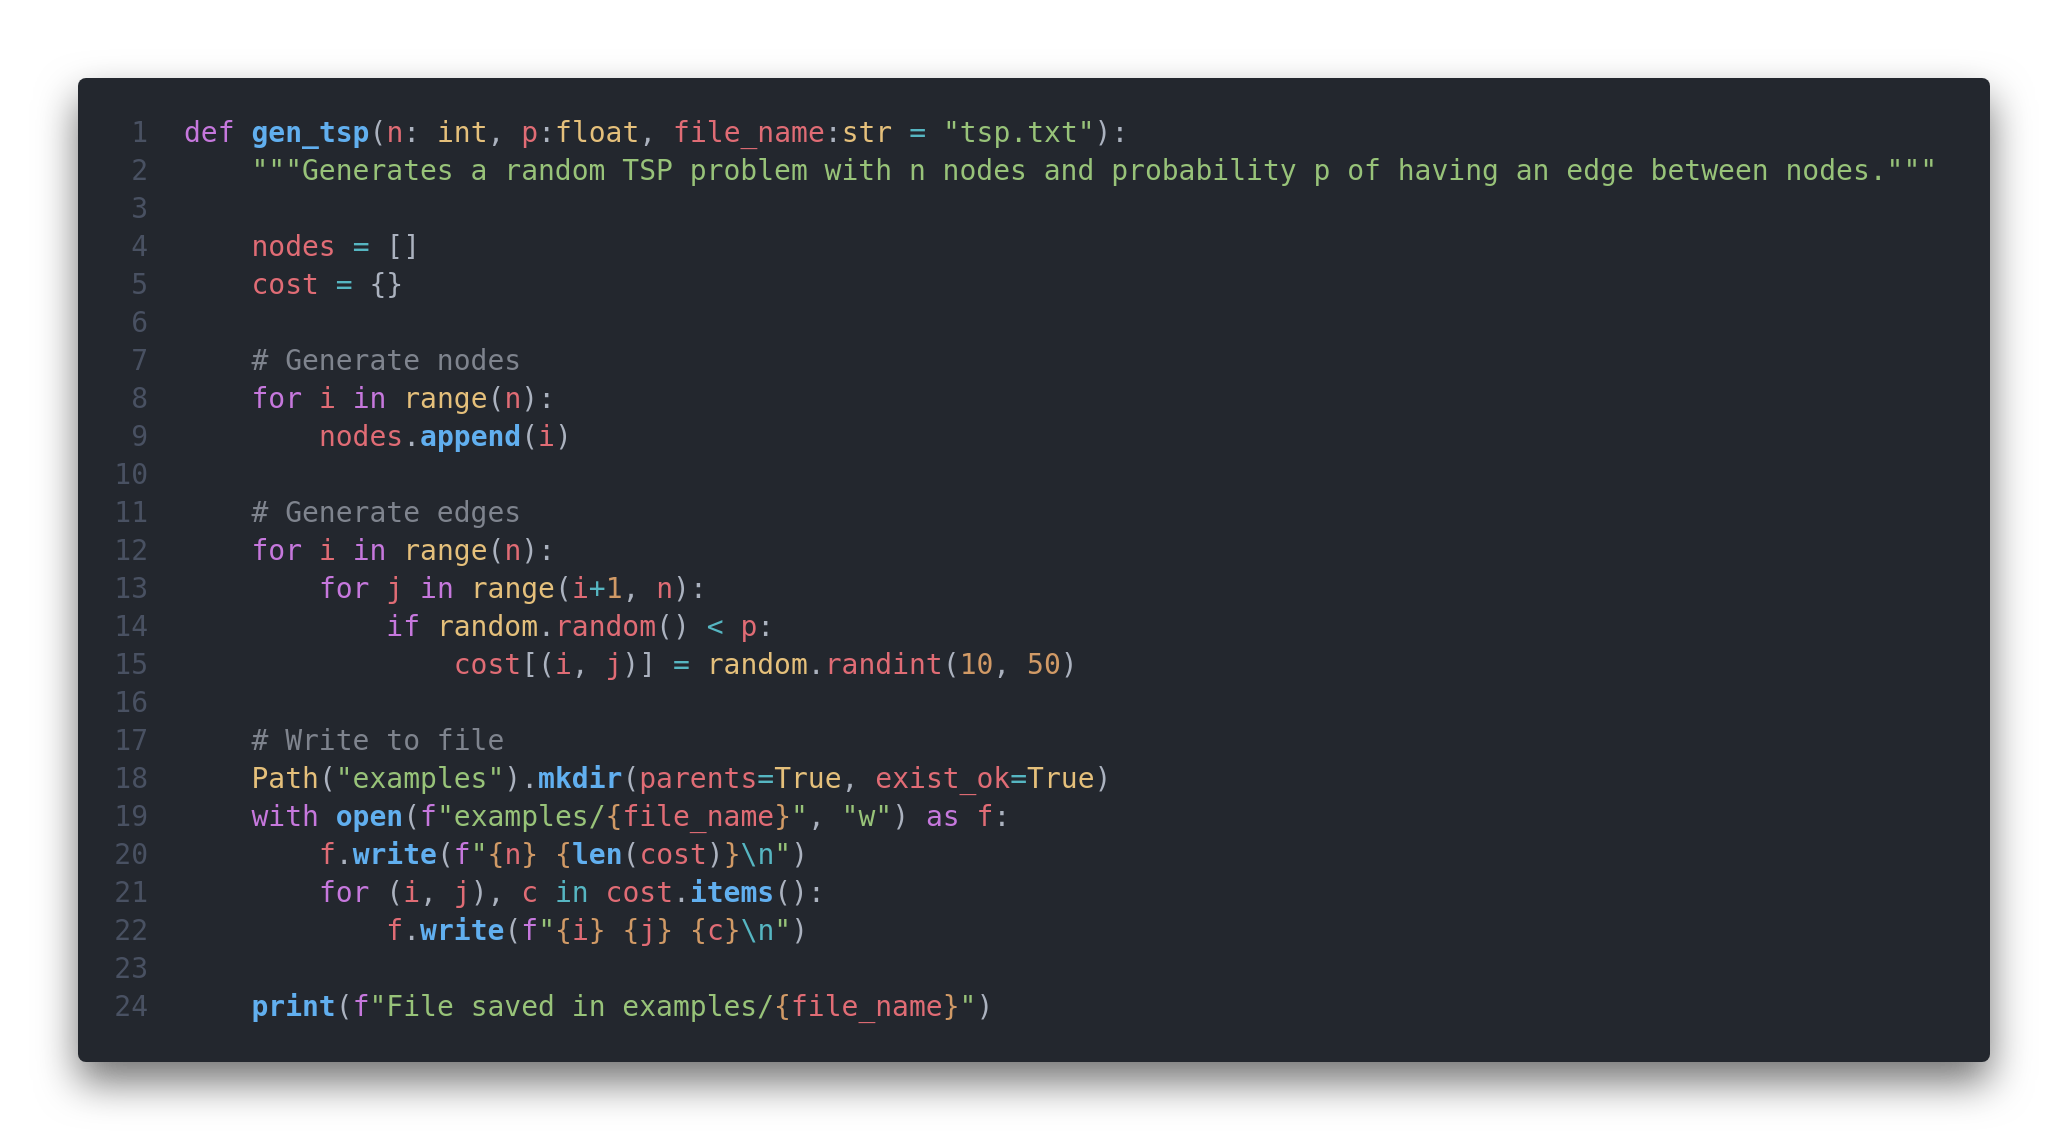
\includegraphics[width=1\textwidth]{resources/gen_tsp.png}
    \caption{Fonction de génération de graphes aléatoires pour le TSP}
    \label{fig:gen_tsp}
\end{figure}

\section*{Résultats et comparaison des méthodes}

Nous pouvons tester nos algorithmes avec un exemple simple fourni par l'énoncé. Ils nous donnent le même résultat :

\begin{figure}[H]
    \centering
    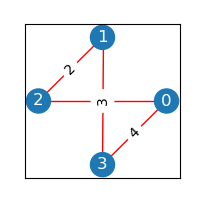
\includegraphics[width=0.5\textwidth]{resources/resol_tsp.png}
    \caption{Résolution d'un exemple simple de TSP}
    \label{fig:resol_bruteforce}
\end{figure}
\newpage

\chapter{Conclusion}
\label{chap:conclusion}

\newpage

\appendix
\pagenumbering{Roman}
\renewcommand{\thepage}{\Roman{page}}

\chapter{Algorithmes et Code}
\section{Plus court chemin}
\label{app:shortest_path_code}

\begin{figure}[H]
    \centering
    \begin{includegraphics}[width=1\textwidth]{resources/path_solver.png}
    \end{includegraphics}
\end{figure}

\section{Modélisation du Problème du Voyageur de Commerce}
\label{app:tsp_model}

\begin{figure}[H]
    \centering
    \begin{includegraphics}[width=1\textwidth]{resources/tsp_solver.png}
    \end{includegraphics}
    
\end{figure}
\newpage

\pagenumbering{arabic}
\renewcommand{\thepage}{\arabic{page}}
\nocite{*}
\printbibliography

\newpage
\end{document}
